\chapter{}

\section{Teori}
 Buat Resume Sejarah Python, perbedaan python 2 dan 3, dengan bahasa yang mudah dipahami dan dimengerti. Buatan sendiri bebas plagiat(10)
 
 Python dikembangkan oleh Guido van Rossum pada tahun 1990 di CWI, Amsterdam sebagai kelanjutan dari bahasa pemrograman ABC. Versi terakhir yang dikeluarkan CWI adalah 1.2.

Tahun 1995, Guido pindah ke CNRI sambil terus melanjutkan pengembangan Python. Versi terakhir yang dikeluarkan adalah 1.6. Tahun 2000, Guido dan para pengembang inti Python pindah ke BeOpen.com yang merupakan sebuah perusahaan komersial dan membentuk BeOpen PythonLabs. Python 2.0 dikeluarkan oleh BeOpen. Setelah mengeluarkan Python 2.0, Guido dan beberapa anggota tim PythonLabs pindah ke DigitalCreations.

Saat ini pengembangan Python terus dilakukan oleh sekumpulan pemrogram yang dikoordinir Guido dan Python Software Foundation. Python Software Foundation adalah sebuah organisasi non-profit yang dibentuk sebagai pemegang hak cipta intelektual Python sejak versi 2.1 dan dengan demikian mencegah Python dimiliki oleh perusahaan komersial. Saat ini distribusi Python sudah mencapai versi 2.6.1 dan versi 3.0.

Nama Python dipilih oleh Guido sebagai nama bahasa ciptaannya karena kecintaan Guido pada acara televisi Monty Python's Flying Circus. Oleh karena itu seringkali ungkapan-ungkapan khas dari acara tersebut seringkali muncul dalam korespondensi antar pengguna Python.
Python juga memmiliki beberapa pembagian,yaitu paython 2 dan 3
\begin{enumerate}
    \item Syntax untuk mencetak teks atau yang lainnya
    \item Syntax untuk meminta inputan
    \item Hasil dari operator pembagian
\end{enumerate}
\section{Resume Implementasi dan penggunaan Python di perusahaan dunia}
Didunia sudah banyak yang menggunakan bahasa pemrograman python untuk perusahaannya diantaranya :
\begin{enumerate}
    \item 
    Spotify merupakan suatu perusahaan penyedia layanan musik streaming yang memanfaatkan bahasa pemrograman python untuk aplikasinya alasannya  service dibuat menggunakan Python dikarenakan Spotify sangat menyukai kecepatan pipeline development.
    \item
    Google merupakan perushaan terbesar didunia yang menggunakan bahasa pemrograman python karena  kemudahan dalam perawatan dalam mengurus programam.
\end{enumerate}

\section{Instalansi Pyton 3}
\begin{enumerate}
    \item Tekan Run untuk melanjutkan instalansi

\begin{figure}[!htbp]
    \centering
    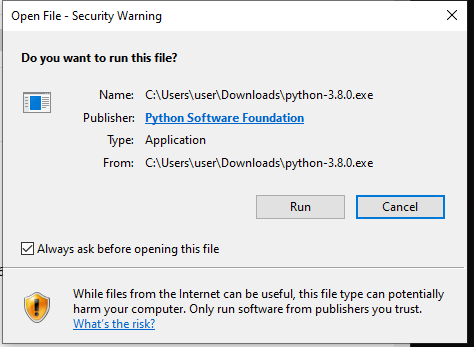
\includegraphics[scale=0.5]{figures/1.png}
    \label{visimisi}
\end{figure}

    \item Tekan Instalansi Now
    \begin{figure}[!htbp]
    \centering
    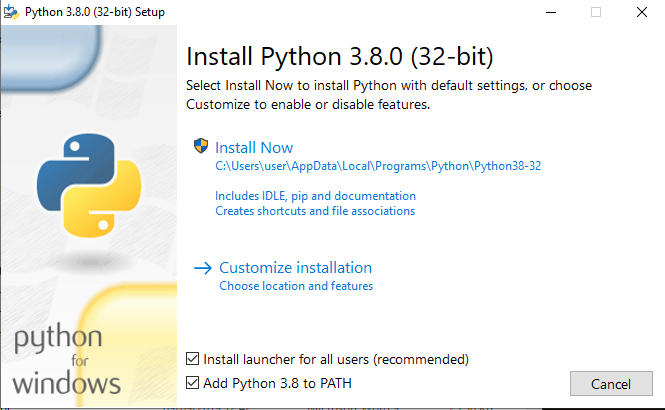
\includegraphics[scale=0.5]{figures/2.png}
    \label{visimisi}
\end{figure}


    \item Tunggu sampai instalansi selesai
    \begin{figure}[!htbp]
    \centering
    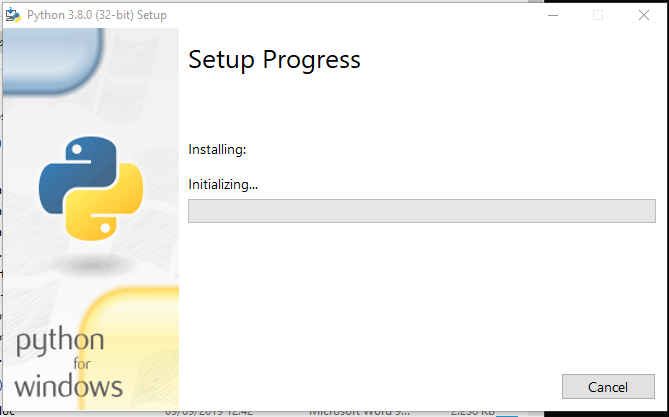
\includegraphics[scale=0.5]{figures/3.png}
    \label{visimisi}
\end{figure}
\end{enumerate}

\section{Instalasnsi Pip}
\begin{enumerate}
    \item Pertama bukalah cmd

\begin{figure}[!htbp]
    \centering
    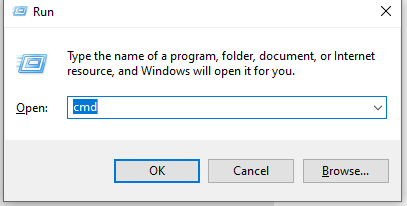
\includegraphics[scale=0.5]{figures/5.png}
    \label{visimisi}
\end{figure}

    \item Pertama bukalah cmd

\begin{figure}[!htbp]
    \centering
    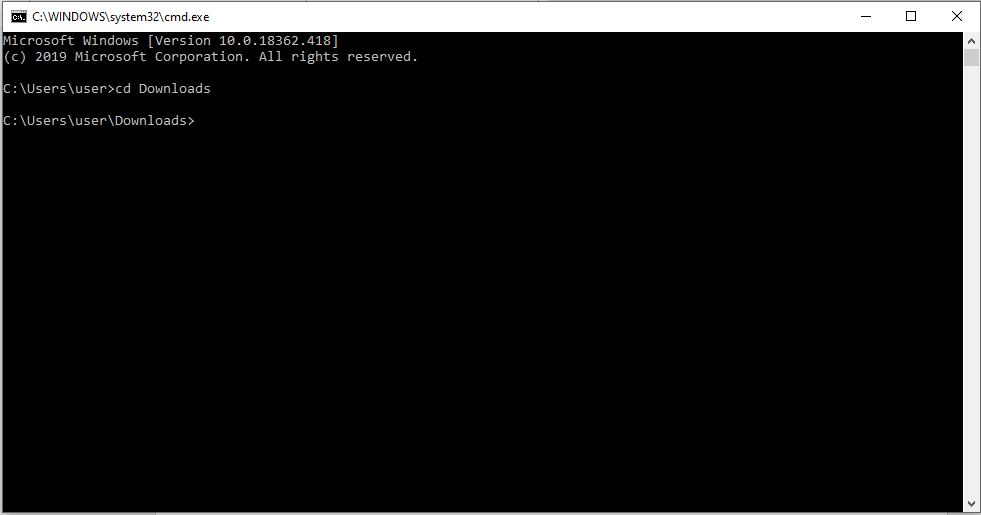
\includegraphics[scale=0.4]{figures/6.png}
    \label{visimisi}
\end{figure}

    \item Pertama bukalah cmd

\begin{figure}[!htbp]
    \centering
    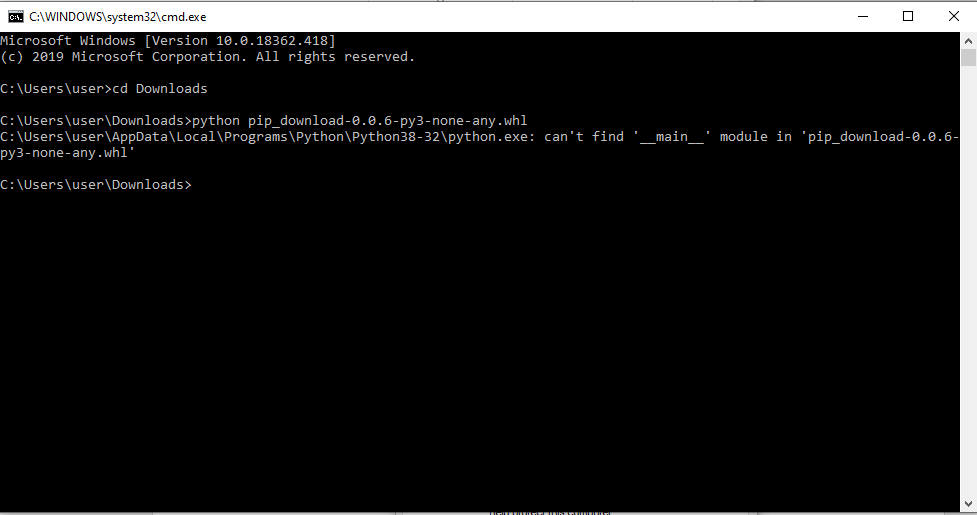
\includegraphics[scale=0.4]{figures/7.png}
    \label{visimisi}
\end{figure}

    \item Ketik cd Dwonloads untuk menentukan lokasi download

\begin{figure}[!htbp]
    \centering
    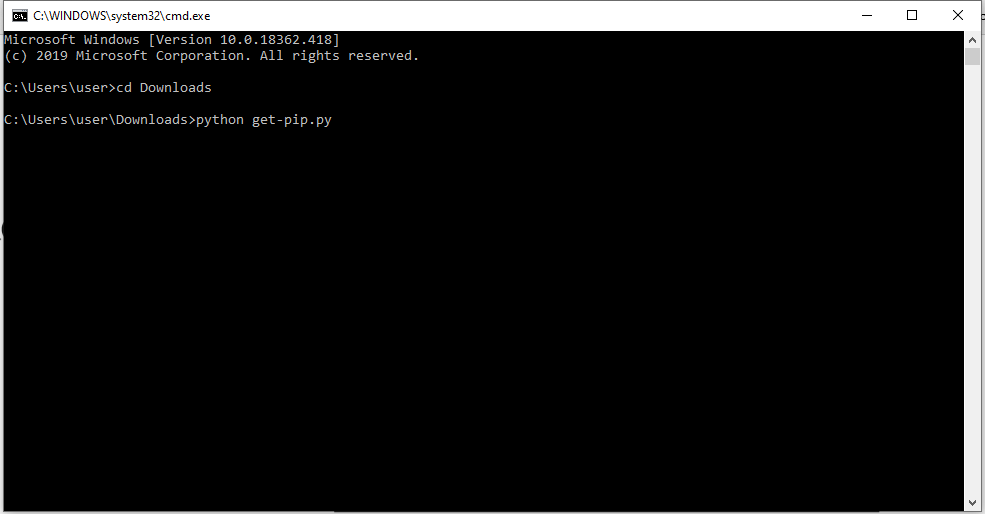
\includegraphics[scale=0.4]{figures/8.png}
    \label{visimisi}
\end{figure}

    \item lalu ketikan cd download (tempat dimana kita menaruh hasil download-an pip)


\begin{figure}[!htbp]
    \centering
    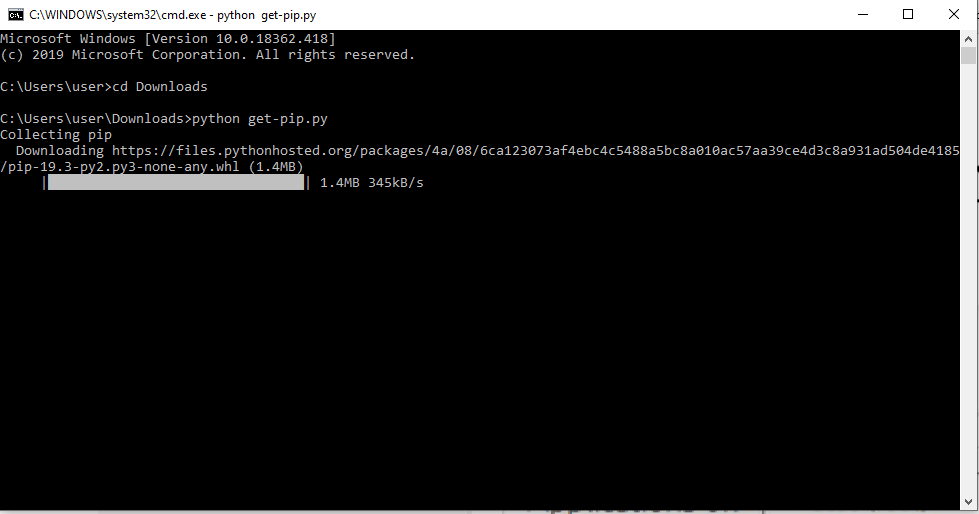
\includegraphics[scale=0.4]{figures/9.png}
    \label{visimisi}
\end{figure}

    \item Tunggu sampai Instalansi selesai

\begin{figure}[!htbp]
    \centering
    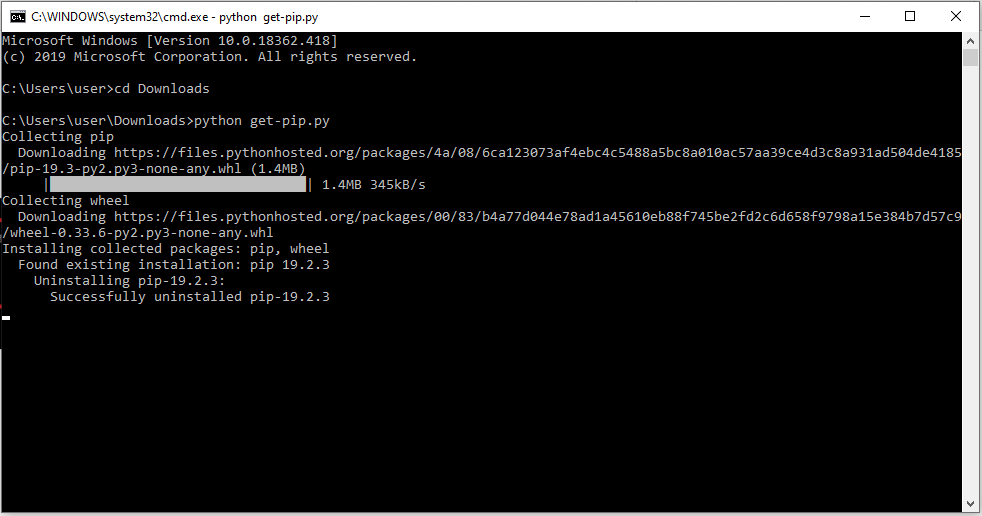
\includegraphics[scale=0.4]{figures/10.png}
    \label{visimisi}
\end{figure}
\end{enumerate}

\section{Entepreter/Cli melalui Terminal}
\begin{enumerate}
    \item Buka file python 3 dan ketik pyton untuk melakukan perintah

\begin{figure}[!htbp]
    \centering
    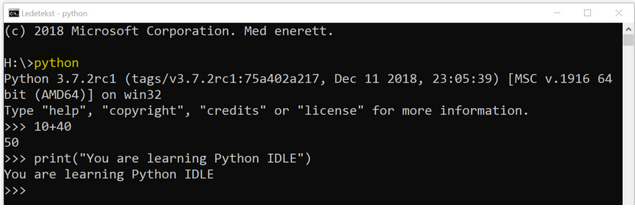
\includegraphics[scale=0.5]{figures/11.png}
    \label{visimisi}
\end{figure}

    \item Ketik lah printah yang anda inginkan

\begin{figure}[!htbp]
    \centering
    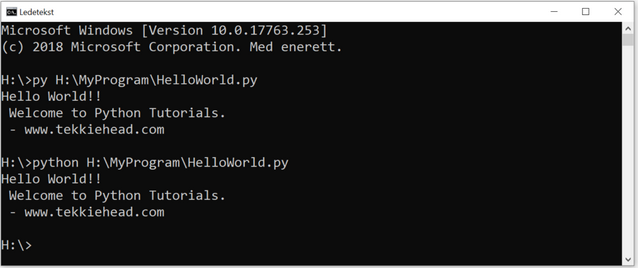
\includegraphics[scale=0.5]{figures/12.png}
    \label{visimisi}
\end{figure}

\end{enumerate}

\section{Menjalankan Script hello word di spyder}
\begin{enumerate}
    \item Buatlah scrip print ("Hellow World!")
\begin{figure}[!htbp]
    \centering
    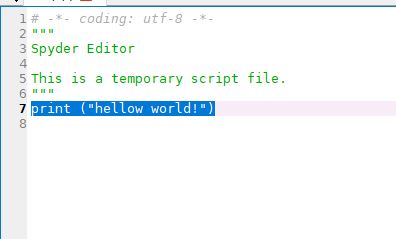
\includegraphics[scale=0.7]{figures/16.png}
    \label{visimisi}
\end{figure}

    \item Setelah selesai tekan lah tanda play 
\begin{figure}[!htbp]
    \centering
    
\includegraphics[scale=0.7]{figures/17.png}
    \label{visimisi}
\end{figure}
     \item Setelah itu akan keluar di consol Hellow World!
\end{enumerate}

\section{Penjelasan Identitas}
Operator identitas adalah operator yang bisa dipakai untuk memeriksa apakah nilai sebuah variabel ada di tempat yang sama (di memory) atau tidak. Operator ini dikenal juga sebagai identity operators.Didalam operator terdapat fungsi,
Fungsi pada Python, dibuat dengan kata kunci def kemudian diikuti dengan nama fungsinya.
    def namafungsi():
    print "Hello ini Fungsi"
    
    Sama seperti blok kode yang lain, kita juga harus memberikan identasi (tab atau spasi 2x) untuk menuliskan isi fungsi.
Kita bisa manfaatkan parameter.Parameter adalah variabel yang menampung nilai untuk diproses di dalam fungsi.Fungsi yang Mengembalikan Nilai
Fungsi yang tidak mengembalikan nilai biasanya disebut dengan prosedur.Namun, kadang kita butuh hasil proses dari fungsi untuk digunakan pada proses berikutnya.
Maka fungsi harus mengembalikan nilai dari hasil pemrosesannya.
Cara mengembalikan nilai adalah menggunkan kata kunci return lalu diikuti dengan nilai atau variabel yang akan dikembalikan.

\section{Jenis jenis error identasi yang didapat}
\begin{enumerate}
    \item Syntax Error,Syntax Error terjadi merupakan jenis kesalahan yang terjadi akibat perintah atau statement yang diketik menyalahi aturan pengkodean oleh bahasa pemrograman yang digunakan. Setiap bahasa pemrograman memiliki aturan pengkodean tersendiri yang harus
    dipatuhi.
    \item Run-time Errorenis, kesalahan Run-time Error terjadi ketika kode program melakukan sesuatu yang tidak dimungkinkan. Contohnya jika pada sebuha aplikasi mencoba mengkases file yang tidak ada, atau terjadi kesalahan alokasi memory.
    \item  Logical Error merupakan jenis kesalahan yang relatif sulit untuk ditemukan penyebabnya. Karena aplikasi yang mnegandung Logical Error berjalan tanpa pesan kesalahan, tetapi mengeluarkan hasil yang tidak diharapkan, misalnya aplikasi yang dibuat menghasilkan perhitungan yang salah.
\end{enumerate}
\section{Cara membaca error}
\begin{enumerate}
    \item Melihat tanda-tanda yang diberikan sistem pada saat eror misal tanda blok merah di scrip yang di jalankan
    \item Melihat console dan mebaca pemberitahuan diconsole mengenai eror dimana dan penyelesaiannya 
\end{enumerate}
\section{Cara menangani error}
Ada dua model penanganan error utama: status code dan exception. Status code dapat digunakan oleh bahasa pemrograman apapun. Exception memerlukan dukungan bahasa/runtime. 
Python mendukung exception. Python dan librari standarnya menggunakan exception secara liberal untuk melaporkan banyak situasi luar biasa seperti IO error, pembagian dengan nol, indexing di luar batas, dan juga beberapa situasi yang tidak begitu luar biasa seperti akhir iterasi (walaupun itu tersembunyi). Kebanyakan librari akan mengikuti kecocokan dan menaikkan exception.

Itu berarti code-mu akan harus menangani exception yang diangkat oleh Python dan librari, sehingga kamu mungkin juga melakukan raise pada exception dari code-mu jika perlu dan tidak bergantung pada status code.
Ada beberapa exception khusus yang diturunkan secara langsung dari BaseException, seperti SystemExit, KeyboardInterrupt dan GeneratorExit. Kemudian ada Exception class, yaitu class dasar untuk StopIteration, StandardError dan Warning. Semua error standard diturunkan dari StandardError.Melakukan raise pada exception sangat mudah. Kamu hanya perlu menggunakan kata kunci raise untuk menaikkan sebuah obyek yaitu sebuah sub-class dari class Exception. Itu dapat berapa sebuah contoh Exception itu sendiri, satu dari exception standar (misalnya RuntimeError), atau sebuah subclass dari Exception yang kamu turunkan sendiri.
Beberapa kegagalan itu sementara, khususnya ketika menangani sistem terdistribusi. Sebuah sistem yang menakutkan pada tanda pertama masalah itu tidak berguna.

Jika code mengakses beberapa sistem jarak jauh yang tidak merespon, solusi tradisional adalah timeout, namun terkadang tidak semua sistem didesain dengan timeout. Timeout tidak selalu mudah untuk dikalibrasi saat kondisi berubah.

Pendekatan lainnya adalah gagal dengan cepat kemudian mencoba ulang. Manfaatnya adalah jika target merespon cepat maka kamu tidak harus menghabiskan banyak waktu dalam kondisi tidur dan dapat bereaksi secara langsung. Namun jika itu gagal, kamu dapat mencoba ulang berkali-kali hingga kita dapat memutuskan itu benar-benar tidak dapat diraih dan menaikkan sebuah exception. Di dalam section berikutnya, saya akan memperkenalkan sebuah decorator yang dapat melakukan itu.

 